\chapter{Public microdata}\label{ch:public}

Every statistical office has files that have been public for a long time. They sit
in teaching packages, on data portals and in the replication archives of journals,
and they are downloaded every week. When an institution designs a new public file,
one of these is often the template, and the argument for it runs as follows. The
older file has been public for years. Thousands of people have used it. If its
records could be linked to named people, someone would have done it and someone
would have said so, and no incident has been reported. Long exposure without harm
is evidence, perhaps the best evidence an institution can get, that a file of that
shape is safe.

The first fact that breaks this argument is about the file, not about its history.
The extract of the US Census 2000 public use sample used in this chapter has been in
teaching use for years. On a key made of four fields that an outsider could plausibly
know, state, area, years of schooling and years of potential experience, 86.3 per
cent of its 29,501 records are unique, and the mean of the reciprocal key frequency
is 0.928.
% source: artifacts-paper/results.json, real.census.full_key (records 29501, unique_share 0.8628, mean_reciprocal_frequency 0.9284); paper/generated/numbers.tex (\runrealuniqueshare 86.3, \runrealmeanrecip 0.928)
Inside the file the key almost determines the record. Whatever has protected the
people behind it, it was not the shape of the file. The second fact is about the
history. An adversary who links a record for gain, curiosity or harm has no reason to
announce it, and the incidents that the field knows about were reported by
researchers who chose to publish them.

This chapter asks one question. What can an attack on a public file tell an
institution about its own confidential register? It runs the pipeline of the
earlier chapters on two real public files, reports what it finds, and then sets out
what such results license and what they do not.

\section{A template for a public extract}

The Bank planned a public extract from its survey of household finances, and the
chair had a suggestion for the release committee. A census teaching file of the same
general shape had been public for years without complaint, she said, and the Bank
could follow its design and save itself a long assessment. Naledi asked for a week.
She would run the Bank's own pipeline on the teaching file and report what a declared
adversary achieved against it. If the file was as safe as its history suggested, the
results would show it.

Her request rested on a distinction the chair accepted at once. A file's history
records what was reported. An assessment records what an attack achieves. The two
coincide only if every successful attack is reported, and the documented cases
suggest the opposite.

\section{What the documented cases show}

The best known re-identification in the literature was an exercise, not a crime.
\citet{sweeney2002} describes how hospital discharge records for state employees in
Massachusetts, released with names removed, were linked to the voter list of
Cambridge through date of birth, sex and postal code, and how the linkage found the
record of the Governor of Massachusetts. The records had already been released; the
linkage became known because the researcher who performed it published it. Her
earlier study \citep{sweeney2000} showed that a few simple demographic fields
identify most people in the United States uniquely, and \citet{golle2006} revisited
that estimate with later census data and found the fields still highly identifying.

\citet{narayanan2008} reached the same kind of result with a different kind of
file. Netflix had released the film ratings of its subscribers, with identities
replaced by numbers, as the data for a public prize. The authors showed that a few
ratings with approximate dates, of the kind people post publicly elsewhere, are
enough to pick out a subscriber's record, and they demonstrated the match against
public ratings on another site. Again the attack became known because its authors
wrote it up. \citet{demontjoye2013} showed that four points in space and time
identify most people in a large mobility data set, and \citet{rocher2019} showed
that releasing only a sample of a population does not prevent a generative model
from estimating, with good accuracy, whether a matched record is the right one.

None of these is evidence that an attack on any particular file has taken place. They
are evidence of something more useful for the present argument: that the files were
open to linkage from the day they were released, and that the world learned of it
only when someone with an interest in publishing chose to publish. Section~\ref{c12:sec-silence}
turns that observation into a statement about how much a quiet history can
show.

\section{Two public files}

The pipeline runs on two files that ship with the \texttt{wooldridge} package for
Python, version 0.5.0, whose contents are identified in the replication record by
their SHA-256 hashes.
% source: artifacts-real/replication.json, source (wooldridge_version 0.5.0; census2000_sha256 ff4ec6f7...; loanapp_sha256 cf4f214c...)
The first is an extract of the US Census 2000 public use microdata sample: 29,501
records with state, public use microdata area, years of schooling, years of
potential experience and log weekly income. The second is the Boston Fed study of
mortgage applications: after dropping incomplete rows, 1,986 applications with area,
applicant income, marital status, dependants, occupancy, the lending decision and a
record of late payments.
% source: src/privacy_risk/realdata.py (load_census2000, load_loan_applications); artifacts-paper/results.json real.loans.structure.records 1986
Both files are already public and already protected. Nothing confidential is read,
and the exercise asks the question an agency asks before publishing a file of that
shape: what would a declared adversary achieve against it?

Three things change when the data are real, and each was a claim of the earlier
chapters. The population behind the file is not observed, so the population
frequency measure cannot be computed and the uniqueness probability has no truth to
be checked against. The analyses that define utility are the ones the file is used
for, not ones the analyst chose. And the risks are far higher than on the synthetic
population of Chapter~\ref{ch:simulation}, so the choice of tolerance bites harder.

The figures in the next sections are prosecutor risks computed inside the file, for
an adversary who knows that its target is in the extract. They are not estimates of
the risk the file posed to the US population, which an office would assess with the
sampling fraction, the population frequencies and the access conditions that this
study does not have.

\section{What the key alone separates}\label{c12:sec-key}

On the full key, the 29,501 census records occupy 27,390 classes. Of those classes
25,454, or 92.9 per cent, hold a single record, and they hold 86.3 per cent of the
records.
% source: artifacts-paper/results.json real.census.full_key (cells 27390, unique_cells 25454, unique_share 0.8628); 25454/27390 = 0.929
The key space, counting the areas actually observed within each state, has 665,896
cells, so the file fills about 4 per cent of it.
% source: artifacts-paper/results.json real.census.key_space 665896; derived 27390/665896 = 0.041
The finding is not that someone blundered. It is that the key an outsider could
reconstruct almost determines the record inside the file, and that any claim that the
file is protected must rest on something other than the key: on the sampling, on what
outsiders actually know, or on the access conditions.

The first of these is the journalist's question of Chapter~\ref{ch:measures}: is a
record unique in the file also unique in the population? On a real file the answer
needs the sampling fraction, which for this extract is not known. The pipeline
assumes $\pi = 0.05$. Under that assumption a negative binomial law fitted to the
observed counts puts the mean population cell at 0.886 people, empty cells included,
and a record unique in the file is unique in the population with probability 0.225.
With the dispersion held at its fitted value, the same calculation gives 0.035 at
$\pi = 0.01$, and lower values at smaller fractions.
% source: artifacts-paper/results.json real.census.journalist (fitted_mean_cell 0.886, rho_model 0.2252); paper/bis_ifc_full.tex Section "The census sample" (0.035 at pi = 0.01)
The file is a small subsample of the 2000 public use sample, so its fraction of the
US population is far below 0.05. The figure of 0.225 is therefore a consequence of an
assumed input and not a finding about the file. Chapter~\ref{ch:simulation} showed
that a fitted law of this kind can be off by a quarter even when its input is right;
here the input is not known, and nothing can be checked. That is the position an
agency is in when it does not know its own sampling fraction, and it is the first
limit on what a public file can show.

\section{A declared attack on the census file}

The pipeline then treats the census file as a candidate release and searches over
protection settings. It plans $3 \times 2 \times 2 \times 3 = 36$ settings, varying the
width of the area, schooling and experience bands and the minimum class size, and
keeps the 25 that retain at least 500 records.
% source: artifacts-paper/config.json real (puma_widths [1,10,100], education_widths [1,4], experience_widths [1,10], min_cell_counts [1,5,10], minimum_release_size 500); paper/generated/numbers.tex \runrealsettings 25
The declared adversary reads the key exactly but allows in its likelihood for a
misreading probability of 0.10, and holds a noisy reading of log weekly income with
standard deviation 0.5. A second adversary reads income twice as precisely. Each is
attacked on 1,500 freshly drawn targets per setting, and the risk reported for a
setting is the larger of the two.
% source: artifacts-real/replication.json real_config (key_error 0.1, covariate_sd 0.5, stronger_covariate_factor 0.5); artifacts-paper/config.json attack_replicates.real 1500

Figure~\ref{c12:fig-audit} sets out the evaluation in the order it runs. The order is
the point. The frontier of settings is chosen after all the attack results are in,
and a bound computed for each setting separately would not survive that choice. The
pipeline therefore computes one exact upper bound for each of the 72 planned
setting and adversary pairs at level $0.05/72$, so that all 72 hold together with
probability at least 0.95 (Proposition~\ref{c12:prop-family}). Any setting chosen
after looking at the results then carries a valid bound.

\begin{figure}[ht]
\centering
\includegraphics[width=0.94\textwidth]{realdata_audit.pdf}
\caption{The public-file evaluation in the order it runs: public files, declared
releases, attack simulation on fresh targets, 72 exact bounds sharing one familywise
error of 0.05, the frontier chosen from them, and sensitivity checks, which lie
outside the family.}
\label{c12:fig-audit}
\end{figure}

\begin{proposition}[A familywise bound survives selection]\label{c12:prop-family}
Let $J$ setting and adversary pairs be planned before any attack is run. For pair $j$,
let $K_j$ be the number of successes in $n_j$ independent attacks with success
probability $p_j$, conditional on the released file and the attack rule, and let
\[
U_j = \begin{cases} B^{-1}_{1-\alpha/J}(K_j+1,\ n_j-K_j), & K_j < n_j,\\ 1, & K_j = n_j,\end{cases}
\]
where $B^{-1}_q(a,b)$ is the $q$ quantile of the beta law. Then
$\Prob\{p_j \le U_j \text{ for all } j\} \ge 1-\alpha$, and for any setting
$\hat\theta$ chosen as a function of all the counts, the reported bound
$\max\{U_j : j \text{ belongs to } \hat\theta\}$ is at least the larger risk of the two
adversaries at $\hat\theta$ on that event.
\end{proposition}

Eight of the 25 settings are nondominated in the plane of the familywise upper bound
and utility, and their bounds run from 0.276 to 0.942.
% source: paper/generated/table_real_census.tex; paper/generated/numbers.tex (\runrealfrontier 8, \runrealrisklow 0.276, \runrealriskhigh 0.942)
Utility charges for coarsening as well as for suppression. Each of the three analyses,
mean income by state, by schooling and by experience, is estimated at the fine level
of its variable, and a release that publishes bands supplies the band mean for every
fine level inside it.
% source: src/privacy_risk/realdata.py utility(); src/privacy_risk/experiments.py real_data() analyses

Figure~\ref{c12:fig-frontier} compares, for the eight frontier settings, the risk the
formula of Chapter~\ref{ch:scenario} gives under exact matching with the simulated
risk of the declared attack and its familywise bound. The simulated attack beats exact
matching at every setting, by a factor between 1.05 and 4.19. At the widest bands with a
minimum class size of ten, which keeps 28 per cent of the records, exact matching gives
0.062 and the simulated attack 0.239.
% source: paper/bis_ifc_full.tex Section "The census sample" (factors 1.05 to 4.19); paper/generated/table_real_census.tex row 1 (kept 0.284, exact 0.0615, simulated 0.2393)

\begin{figure}[ht]
\centering
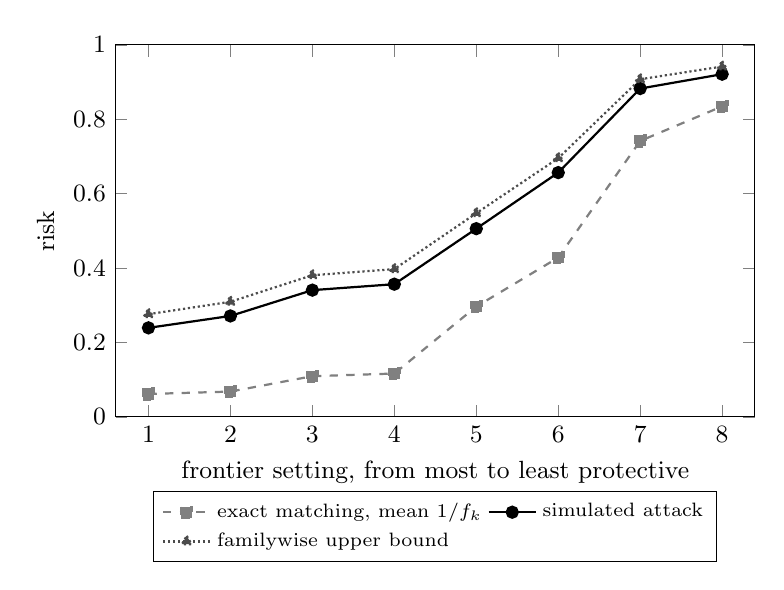
\begin{tikzpicture}
\begin{axis}[width=0.8\textwidth,height=0.52\textwidth,
  xmin=0.6,xmax=8.4, ymin=0,ymax=1,
  xtick={1,2,3,4,5,6,7,8},
  xlabel={frontier setting, from most to least protective}, ylabel={risk},
  legend style={at={(0.5,-0.2)},anchor=north,legend columns=2,font=\scriptsize}, legend cell align=left,
  tick label style={font=\small},label style={font=\small}]
\addplot[thick,black!50,dashed,mark=square*] coordinates
  {(1,0.0615) (2,0.0680) (3,0.1093) (4,0.1165) (5,0.2965) (6,0.4282) (7,0.7418) (8,0.8348)};
\addlegendentry{exact matching, mean $1/f_k$}
\addplot[thick,black,solid,mark=*] coordinates
  {(1,0.2393) (2,0.2713) (3,0.3407) (4,0.3567) (5,0.5060) (6,0.6567) (7,0.8827) (8,0.9213)};
\addlegendentry{simulated attack}
\addplot[thick,black!70,densely dotted,mark=triangle*] coordinates
  {(1,0.2761) (2,0.3094) (3,0.3808) (4,0.3972) (5,0.5475) (6,0.6954) (7,0.9077) (8,0.9419)};
\addlegendentry{familywise upper bound}
\end{axis}
\end{tikzpicture}
\caption{The eight nondominated settings for the census extract. Settings 1 to 4 apply
a minimum class size of 10 or 5 with wide bands; settings 5 to 8 suppress nothing and
narrow the bands in turn. The attack that uses a noisy reading of income beats exact
matching on the key at every setting. Series differ by line style and marker as well
as shade.}
\label{c12:fig-frontier}
\end{figure}
% source for all points: paper/generated/table_real_census.tex

These are conditional attack success rates against the tested public file, not
population re-identification rates and not certificates against attacks that were not
tested. The pipeline also reads implied tolerances off this frontier, in the manner of
Chapter~\ref{ch:tolerance}, and the book does not report them: a tolerance for a file of
this kind is a policy choice for the office that publishes it, and in-file prosecutor
risks are not the quantity it would govern.

Naledi's note to the chair after the first run was short. The template file, judged by
the Bank's own method, had a declared-attack risk above one fifth at every setting the
pipeline could find, and above one half at every setting that suppressed nothing.
% source: paper/generated/table_real_census.tex (simulated column: all >= 0.2393; k_min = 1 rows all >= 0.5060)
Its history said nothing about that, because nothing in its history measured it.

\section{How much the attacker's knowledge moves the figure}

The figures above assume one reading precision. The attacker's knowledge is an input,
and an exploratory run makes its weight visible. On one setting of the census grid,
with 3,000 targets per level, the declared attack succeeds with probability 0.371,
0.271 and 0.186 as the standard deviation of its log-income reading rises from 0.25
to 0.5 to 1.0. On the mortgage file the corresponding rates are 0.179, 0.137 and 0.093
for loan-amount readings with standard deviations of 20, 40 and 80.
% source: artifacts-real/replication.json exploratory_sensitivity (0.3707, 0.2713, 0.1860; 0.1793, 0.1370, 0.0933); docs/REAL_DATA_PROVENANCE.md
These rates come from an archived run and carry individual 95 per cent intervals only;
they lie outside the 72-comparison family. Cutting the error of the attacker's
reading by a factor of four doubles its success on the census file,
% derived: 0.371/0.186 = 1.99
 and the figure an institution reports is
therefore a statement about the attacker as much as about the file. That is why the
decision record of Chapter~\ref{ch:thresholds} names the adversary beside the number.

\section{The worst records}

The decision rule of Chapter~\ref{ch:decision} is stated for every target in a declared
set, and on a real file the worst records are easy to find. The pipeline takes the
middle setting of the census frontier, with areas grouped in hundreds, four-year
schooling bands, ten-year experience bands and no minimum class size, and examines 80 records that sit in classes
of one. The attack names them with mean probability 1.000; the worst is identified with
probability 1.00 and a lower bound, corrected for selection as in
Proposition~\ref{c11:prop-worst}, of 0.964.
% source: artifacts-paper/results.json real.census.worst_target (targets 80, smallest_cell 1, mean 0.99994, maximum 1.0, maximum_lower_bound 0.9638); paper/generated/numbers.tex (\runrealworsttargets, \runrealworstmean, \runrealworst, \runrealworstlower)
On this setting the key alone separates them, so the check shows how exposed an
unsuppressed release of the file is. It does not test a $k$-anonymity promise, since the
setting makes none, and it should not be set beside the synthetic result of
Section~\ref{c11:sec-kanon}.

\section{Pooled releases from the census file}

Chapter~\ref{ch:programmes} reported, in one sentence, that the gap between pooled and
marginal risk appears on real data as well as on synthetic data. The census file is
where it was measured. Four releases are built from it, each with a minimum class size
of three: geography and schooling; geography and experience; state, schooling and
experience; and the full key with experience in ten-year bands. As in the synthetic
study, the releases are taken to share a record identifier, so that a record can be
matched across them.
% source: src/privacy_risk/experiments.py real_data() plans; artifacts-paper/results.json real.census.composition (minimum_cell 3, targets 5000)
Four public-use files cut from one census sample would not ordinarily carry a common
identifier, and an adversary would then have to link them through the published
fields. That case was not measured.

Figure~\ref{c12:fig-pool} shows the result for 5,000 targets. The marginal risks are
0.138, 0.030, 0.118 and 0.096. The second release keeps only 2,812 of the 29,501
records, because geography with single years of experience leaves most classes below
three, which is why its marginal risk is small. The marginals bound the chance that
any one release succeeds between 0.138 and 0.381, and independence would give 0.332.
% source: artifacts-paper/results.json real.census.composition (marginal [0.1376, 0.0296, 0.1178, 0.0956], releases[1].released 2812, marginal_lower 0.1376, union_upper 0.3805, independence 0.3322)

\begin{figure}[ht]
\centering
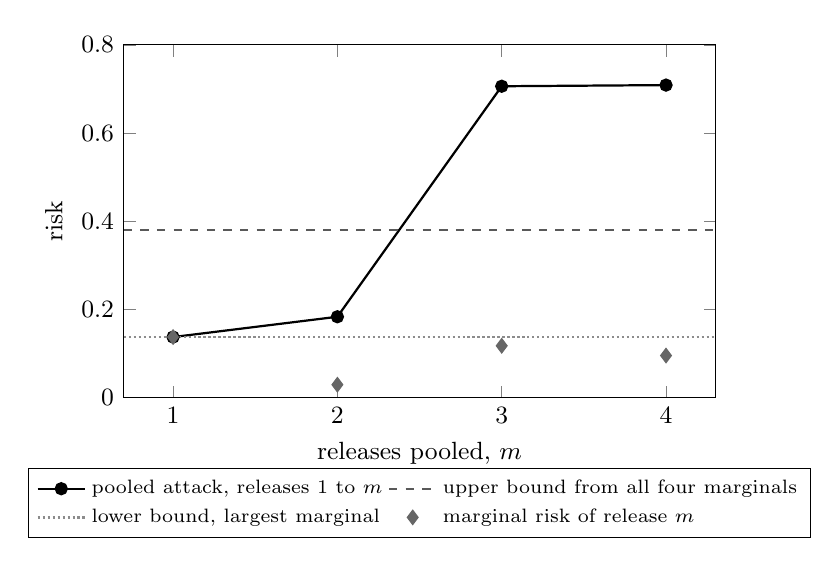
\begin{tikzpicture}
\begin{axis}[width=0.75\textwidth,height=0.5\textwidth,
  xmin=0.7,xmax=4.3, ymin=0,ymax=0.8, xtick={1,2,3,4},
  xlabel={releases pooled, $m$}, ylabel={risk},
  legend style={at={(0.5,-0.2)},anchor=north,legend columns=2,font=\scriptsize}, legend cell align=left,
  tick label style={font=\small},label style={font=\small}]
\addplot[thick,black,solid,mark=*] coordinates {(1,0.1376) (2,0.1836) (3,0.7063) (4,0.7089)};
\addlegendentry{pooled attack, releases $1$ to $m$}
\addplot[thick,black!65,dashed,domain=0.7:4.3,samples=2] {0.3805};
\addlegendentry{upper bound from all four marginals}
\addplot[thick,black!45,densely dotted,domain=0.7:4.3,samples=2] {0.1376};
\addlegendentry{lower bound, largest marginal}
\addplot[only marks,mark=diamond*,mark size=2.6pt,black!60] coordinates {(1,0.1376) (2,0.0296) (3,0.1178) (4,0.0956)};
\addlegendentry{marginal risk of release $m$}
\end{axis}
\end{tikzpicture}
\caption{Four 3-anonymous releases from the census extract, assumed to share a record
identifier, 5,000 targets. The pooled attack leaves the interval implied by the
marginals once the third release is added. Series differ by line style and marker as
well as shade.}
\label{c12:fig-pool}
\end{figure}
% source: artifacts-paper/results.json real.census.composition (pooled [0.1376, 0.1836, 0.7063, 0.7089], marginal, union_upper)

The pooled attack reaches 0.709 with all four releases, 1.86 times the upper bound, and
60.7 per cent of targets are identified uniquely by the intersection although no
release contains a unique record.
% source: paper/generated/numbers.tex (\runrealpooled 0.709, \runrealpooledratio 1.86, \runrealpooledunique 60.7)
The shape of the curve explains the mechanism. The first two releases together add
little, 0.184, because the second covers so few records. The jump comes with the third:
the first release carries the area and the third carries experience, and between them
they rebuild almost the whole key, which Section~\ref{c12:sec-key} showed to be nearly
unique. This is the remark of Chapter~\ref{ch:programmes} in a concrete form. Releases
that share an identifier are one release keyed on the union of their keys, and here the
union is the full key.
% source: artifacts-paper/results.json real.census.composition (pooled[1] 0.1836, unique_share [0, 0.0322, 0.607, 0.607])

On the synthetic population the same comparison gave 1.8 times the bound. Each figure
comes from one draw, so the two do not show that the effect is larger on either kind of
data. They show that it is not an artefact of synthetic data.

\section{The mortgage applications}

The second file is small and makes concrete three risks that the census file does not.
On the key of area, income band, marital status, dependants and occupancy, the 1,986
applications occupy 150 classes, of which 63, or 42 per cent, are unique; those classes
hold 3.2 per cent of the applications. An adversary holding a noisy reading of the loan
amount, with standard deviation 40 in the file's units, identifies 0.134 of applications
over 1,500 attacks, with a one-sided upper bound of 0.149.
% source: artifacts-paper/results.json real.loans.structure (cells 150, unique_cells 63, unique_share 0.0317) and real.loans.identification (rate 0.134, trials 1500, upper 0.1493); src/privacy_risk/experiments.py (covariate sd 40.0)

Attribute disclosure is the risk this file shows most clearly. 12.2 per cent of
applications sit in a class where every application received the same decision, and
0.65 per cent sit in a class where every application was denied, so for those applicants
the denial is disclosed by the class without any record being identified. For late
payments the shares are 29.6 per cent and 0.35 per cent.
% source: artifacts-paper/results.json real.loans.denied (homogeneous_share 0.1224, homogeneous_positive_share 0.00655) and real.loans.late (0.2961, 0.00352); paper/generated/numbers.tex (\runloandeniedhomogeneous, \runloandeniedpositive, \runloanlatehomogeneous, \runloanlatepositive)
Both harmful directions occur here, where the synthetic credit register of
Chapter~\ref{ch:credit} had none, which is the difference between a base rate chosen for
a simulation and one that occurred.

Published totals leak by subtraction. Aggregating loan amounts by area, occupancy and
income band gives 48 cells, of which 16, a third, contain a single application, so that
application's amount is the published total. Those cells hold 2.2 per cent of the
lending in the file, and a rule requiring three records per cell would suppress 20 of
the 48 cells, 42 per cent of them.
% source: artifacts-paper/results.json real.loans.residual[0] (cells 48, single_record_cells 16, exposed_amount_share 0.0223, cells_below_minimum 20, share 0.4167)
The file was designed for the study of lending discrimination and serves it well. The
point of these figures is that the same table, published by an agency without an
assessment, would have disclosed the amounts of sixteen individual applications.

\section{Models fitted on the public file}

The repository also holds two exploratory runs that fit models to attack outcomes on
the census file, holding out whole states for testing, as a check on the proposal models
of Chapter~\ref{ch:proposals}. On three overlapping state-held-out splits, the held-out
binomial log loss of a linear logistic model is between 0.607 and 0.621, and a logistic
model with quadratic terms does slightly better than one- and three-layer networks on
every split, at between 0.602 and 0.614.
% source: paper/generated/table_real_neural.tex; artifacts-real/neural_comparison.json
The differences are in the third decimal place. These runs predict one declared attack on
public data, the models were never trained on final audit outcomes, and their predictions
are not risk bounds. Chapter~\ref{ch:proposals} discusses what such models are for and
reports the negative results beside the positive ones; nothing in this chapter rests on
them.

\section{What a quiet history can show}\label{c12:sec-silence}

The chair's argument can now be put in a form that can be tested. Suppose attempts to
link the file's records to named people arrive over time at some rate, each succeeds
with the probability the file's risk gives, and each success becomes publicly known with
some probability. The institution observes the number of reported incidents. How far
should a count of zero over many years move its belief that the file is safe?

\begin{proposition}[A quiet history is weak evidence]\label{c12:prop-silence}
Suppose attempts arrive as a Poisson process of rate $\lambda$ per year, each succeeds
independently with probability $p$, and each success is reported independently with
probability $r$. Compare the hypotheses that the file's risk is $p_0$ and that it is
$p_1 > p_0$. After $T$ years with no reported incident, the posterior odds of the second
hypothesis are at least
\begin{equation}\label{c12:eq-silence}
\frac{\Prob(p_1)}{\Prob(p_0)}\,\exp\{-\lambda r T (p_1 - p_0)\}
\ \ge\ \frac{\Prob(p_1)}{\Prob(p_0)}\,e^{-\lambda r T}.
\end{equation}
In particular, as the reporting probability $r$ tends to zero the quiet history leaves
the prior odds unchanged, whatever the number of years and the rate of attempts.
\end{proposition}

The proposition says that a quiet history is evidence of safety only in proportion to
$\lambda r T$, the expected number of reported attempts. Every factor in that product is
uncertain, and one of them is likely to be small. The adversaries a release committee
most needs to worry about, a lender reading a competitor's customers, a fraudster, a
journalist with a story not yet written, gain nothing from announcing a successful link
and may lose a great deal. The documented cases were reported by researchers who wanted
them known. A file can be open to linkage for years, as the Netflix ratings and the
Massachusetts hospital records were, and become known as such only on the day someone
chooses to say so.

The proposition also says what would make the history informative. If an institution
monitored the uses of its file, required registration for access, or ran periodic attacks
of its own and published the results, the reporting probability would rise and a quiet
history would start to carry weight. That is a design choice for the access route, and it
is one reason the decision record of Chapter~\ref{ch:thresholds} names the route.

\section{What public files can and cannot show}

The chapter asked what an attack on a public file can tell an institution about its own
confidential register. The answer has a positive part and a limiting part.

The positive part is that a public file is a real file with a real distribution, and the
pipeline's findings on synthetic data reappear on it. A covariate the adversary reads
beats exact matching at every setting. When releases share an identifier, the pooled
attack leaves the interval the marginals imply. Attribute disclosure and leakage by
subtraction occur at rates that nobody chose. These are findings about files of that
shape, and an institution designing a file of the same shape learns from them which
attacks to run and roughly how strong they are.

The limiting part has four elements. The population behind a public file is not observed,
so the uniqueness probability rests on an assumed sampling fraction and a fitted law that
cannot be checked, and utility is measured against the file and not against the
population. The adversary is declared and not observed: the misreading rate and the
precision of the income reading are assumptions, and the attacker's knowledge moves the
risk by a factor of two. The files are public, so the exercise measures what a release of
that shape discloses and says nothing about whether a wrong was done in publishing them.
And only the demographic path of the pipeline has run on them; the credit evaluation of
Chapter~\ref{ch:credit} has run only on the synthetic register.

Together these limits say that a public file can teach an institution which attacks to
run, but cannot run them for it. The confidential register has its own key, its own
population and its own adversaries, and the assessment must be done on it. A long
history without reported incident adds little, because the people most able to exploit a
file are the least likely to report having done so.

Naledi's report to the committee said this in four sentences. The template file was
highly identifying on a key an outsider could know. Its history was silent because nobody
had an interest in speaking. The Bank's extract would be assessed on the Bank's survey,
with the Bank's own adversaries declared. And the template was useful for one thing: it
showed which attacks to run first. The chair accepted the report. When Grace read the
decision record, the line that cited the template file had been replaced by the name of
the adversary the Bank had assessed, and the template was cited only as the source of the
attack design.

\begin{inpractice}[In practice: using a public file as a template]
Do not cite a file's public history as evidence that a release of the same shape is safe;
a quiet history is evidence only in proportion to the expected number of reported
attempts, which is rarely known and often small. Use the public file to choose and test
attacks: run the declared attack on it, with and without each auxiliary field, and with
several precisions for the adversary's readings. Bound every setting in the grid together
before choosing among them. Check attribute homogeneity and published totals as well as
identification. Then repeat the assessment on the confidential register, and record which
results came from the template and which from the register.

\sloppy\smallskip\noindent\textit{In the software.} The two files are loaded by
\texttt{privacy\_risk.realdata} (\texttt{load\_census2000},
\texttt{load\_loan\_applications}); releases are built by \texttt{build\_release} and
attacked by \texttt{attack} and \texttt{per\_target}. Attribute and residual disclosure are
\texttt{attribute\_disclosure} and \texttt{residual\_disclosure}, and the pooled attack is
\texttt{composition}, which calls \texttt{composition.pooled\_attack\_from\_sets}. The whole
study is \texttt{experiments.real\_data}, and \texttt{scripts/realdata\_replication.py}
reruns it with source hashes and the sensitivity checks. The familywise level is set in
one place:
\begin{lstlisting}
grid_size = (len(settings.get("puma_widths", [1, 10, 100]))
             * len(settings.get("education_widths", [1, 4]))
             * len(settings.get("experience_widths", [1, 10]))
             * len(settings.get("min_cell_counts", [1, 5, 10])))
family_alpha = alpha / (2 * grid_size)
\end{lstlisting}
\end{inpractice}

\section{Proofs}

\begin{proof}[Proof of Proposition~\ref{c12:prop-family}]
Fix $j$ and write $b = n_j$, $k = K_j$, $\gamma = \alpha/J$, and
$F_p(k) = \sum_{s=0}^{k}\binom{b}{s}p^s(1-p)^{b-s}$. For $k < b$, $F_p(k)$ is continuous
and strictly decreasing in $p$, and the binomial and beta laws are linked by
$F_p(k) = 1 - I_p(k+1, b-k)$, so $U_j$ is the unique solution of $F_{U_j}(k) = \gamma$.
For a fixed true $p_j$, the event $\{U_j < p_j\}$ therefore equals
$\{F_{p_j}(K_j) < \gamma\}$, which is a lower tail $\{K_j \le k_\ast\}$ of the count
because $F_{p_j}(k)$ increases in $k$. Its probability is $F_{p_j}(k_\ast) < \gamma$,
or zero if the tail is empty; when $K_j = b$ the bound is 1 and cannot fail. Hence
$\Prob\{p_j > U_j\} \le \gamma$ for every $j$.

By the union bound,
$\Prob\{\exists j : p_j > U_j\} \le J\gamma = \alpha$, with no assumption about how the
counts for different pairs depend on one another. On the complementary event, every
inequality $p_j \le U_j$ holds at once. A setting $\hat\theta$ chosen from the counts is
one of the planned settings, so both of its pairs are among the $J$, and the larger of its
two risks is at most the larger of its two bounds. Selection cannot move the realised
counts off the event on which all bounds hold, so the guarantee is unaffected by it.
\end{proof}

\begin{proof}[Proof of Proposition~\ref{c12:prop-silence}]
Attempts form a Poisson process of rate $\lambda$, and each is independently a reported
success with probability $pr$. By the thinning property of the Poisson process, reported
incidents form a Poisson process of rate $\lambda p r$, so the number $N$ reported in $T$
years is Poisson with mean $\lambda p r T$, and
$\Prob(N = 0 \mid p) = \exp(-\lambda p r T)$. Bayes' rule in odds form gives
\[
\frac{\Prob(p_1 \mid N = 0)}{\Prob(p_0 \mid N = 0)}
= \frac{\Prob(p_1)}{\Prob(p_0)}\cdot\frac{e^{-\lambda p_1 r T}}{e^{-\lambda p_0 r T}}
= \frac{\Prob(p_1)}{\Prob(p_0)}\,\exp\{-\lambda r T(p_1 - p_0)\}.
\]
Since $0 \le p_0 < p_1 \le 1$, the difference $p_1 - p_0$ is at most one, which gives the
second inequality in \eqref{c12:eq-silence}. As $r \to 0$ the exponential factor tends to
one for fixed $\lambda$ and $T$, so the posterior odds tend to the prior odds.
\end{proof}
